\chapter{重力与质量}\label{ch:g4:weight-and-mass}

宇航员在\omterm{def:g2:moon-in-the-sky:moon}{月球}上像孩子在蹦床上一样弹跳，
尽管他们背着很重的背包。他们的背包在那里是重还是轻？
要想好好回答，我们得把日常用语“重”一分为二：
一是物体\emph{由什么构成}——即其\omterm{def:g3:measuring-mass:mass}{质量}；二是地球
\emph{拉它的力有多大}——即其\omterm{def:g4:weight-and-mass:weight}{重力}。两者关系密切，像是表亲，
却不是双胞胎。

\section{藏在“重”字里的两个概念}

你知道\omterm{def:g3:measuring-mass:mass}{质量}：物体所含物质的多少，用克和\omterm{def:g3:measuring-mass:units}{千克}计量，
可用\omterm{def:g3:levers-and-scales:scale}{天平}来比较。你也知道地球的拉力：一种不接触的
力，使每件被松手的东西都向下落。
\omterm{def:g4:weight-and-mass:weight}{重力}正是两者的交汇处。

\begin{definition}[重力]\label{def:g4:weight-and-mass:weight}
物体的\emph{重力}\index{重力}，是地球向下拉它的
力。提着水桶时，手臂要对抗的正是重力，
挂着水桶时，拉长弹簧的也是重力。
和所有的力一样，重力有方向：始终
竖直向下。
\end{definition}

\begin{proposition}[物质越多，拉力越大]\label{prop:g4:weight-and-mass:morestuff}
地球对所含物质越多的物体拉得越用力：在
同一地点，\omterm{def:g3:measuring-mass:mass}{质量}越大，\omterm{def:g4:weight-and-mass:weight}{重力}必定越大——两块
相同的砖块，\omterm{def:g4:weight-and-mass:weight}{重力}是一块的两倍。这就是\omterm{def:g3:levers-and-scales:scale}{天平}——
通过比较两个托盘上的\emph{拉力}，
能够比较\emph{\omterm{def:g3:measuring-mass:mass}{质量}}：同一地点，拉力相等即物质相等。
\end{proposition}

\begin{example}[表亲而非双胞胎]\label{ex:g4:weight-and-mass:cousins}
\omterm{def:g3:measuring-mass:mass}{质量}回答的是：\emph{物质有多少？}它只取决于物体本身，
无论在手里、水下还是\omterm{def:g2:moon-in-the-sky:moon}{月球}上都一样。\omterm{def:g4:weight-and-mass:weight}{重力}回答的是：
\emph{这里它被拉得有多用力？}它既取决于
物体本身，\emph{以及}它所处的位置。只改变地点，
\omterm{def:g3:measuring-mass:mass}{质量}不变，\omterm{def:g4:weight-and-mass:weight}{重力}却可能改变。
\end{example}

\section{弹簧测力计}

\begin{definition}[弹簧测力计]\label{def:g4:weight-and-mass:springscale}
\emph{弹簧测力计}\index{弹簧测力计}通过让物体拉伸弹簧
来\omterm{def:g2:measuring-length:measure}{测量}\omterm{def:g4:weight-and-mass:weight}{重力}：拉力越大，弹簧伸得越长。
弹簧旁边的指针指示出读数。
钓鱼用的秤、行李秤，以及厨房秤的内部结构，
都是这样工作的——它们感知的是\emph{拉力}，而不是物质。
\end{definition}

\begin{omfigure}
\begin{tikzpicture}[scale=0.85]
  \draw[thick] (0.6,4.2) -- (2.2,4.2);
  \draw[thick] (1.4,4.2) -- (1.4,3.9);
  \draw[thick] (1.4,3.9) .. controls (1.7,3.75) and (1.1,3.6)
    .. (1.4,3.45) .. controls (1.7,3.3) and (1.1,3.15) .. (1.4,3.0);
  \draw[thick] (1.4,3.0) -- (1.4,2.7);
  \draw[thick, fill=omMeth, fill opacity=0.4]
    (1.0,2.0) rectangle (1.8,2.7);
  \node[right, font=\footnotesize] at (1.95,2.35) {$1$ 块砖};
  \draw[thick] (5.6,4.2) -- (7.2,4.2);
  \draw[thick] (6.4,4.2) -- (6.4,3.9);
  \draw[thick] (6.4,3.9) .. controls (6.7,3.68) and (6.1,3.47)
    .. (6.4,3.25) .. controls (6.7,3.03) and (6.1,2.82) .. (6.4,2.6)
    .. controls (6.7,2.38) and (6.1,2.17) .. (6.4,1.95);
  \draw[thick] (6.4,1.95) -- (6.4,1.7);
  \draw[thick, fill=omMeth, fill opacity=0.4]
    (6.0,0.3) rectangle (6.8,1.0);
  \draw[thick, fill=omMeth, fill opacity=0.4]
    (6.0,1.0) rectangle (6.8,1.7);
  \node[right, font=\footnotesize] at (6.95,1.0) {$2$ 块砖};
  \node[right, font=\small] at (8.0,3.4)
    {质量加倍，};
  \node[right, font=\small] at (8.0,2.9)
    {拉力加倍，};
  \node[right, font=\small] at (8.0,2.4)
    {伸长加倍};
\end{tikzpicture}

{\small 弹簧能感知\omterm{def:g4:weight-and-mass:weight}{重力}：一块砖使它伸长；两块相同的
砖使它伸长的距离是原来的两倍。}
\end{omfigure}

\begin{method}[橡皮筋测力计]\label{met:g4:weight-and-mass:rubberband}
自己动手做一个测\omterm{def:g4:weight-and-mass:weight}{重力}的小装置：
\begin{enumerate}
  \item 把橡皮筋挂在挂钩上，
        并在其底部粘上一个轻的纸杯；
  \item 杯子为空时，标出杯口的位置，
        先不\omterm{def:g2:measuring-length:measure}{测量}：这就是零刻度。
  \item 往杯中放入 $10$ 颗弹珠（比如），并用
        尺子量出杯口比零刻度低了多少；
  \item 再放入 $20$ 颗弹珠，重新\omterm{def:g2:measuring-length:measure}{测量}。
\end{enumerate}
弹珠数量加倍，伸长量大约也加倍：你的橡皮筋
证实了命题——物质越多，拉力越大。
\end{method}

\begin{omfigure}
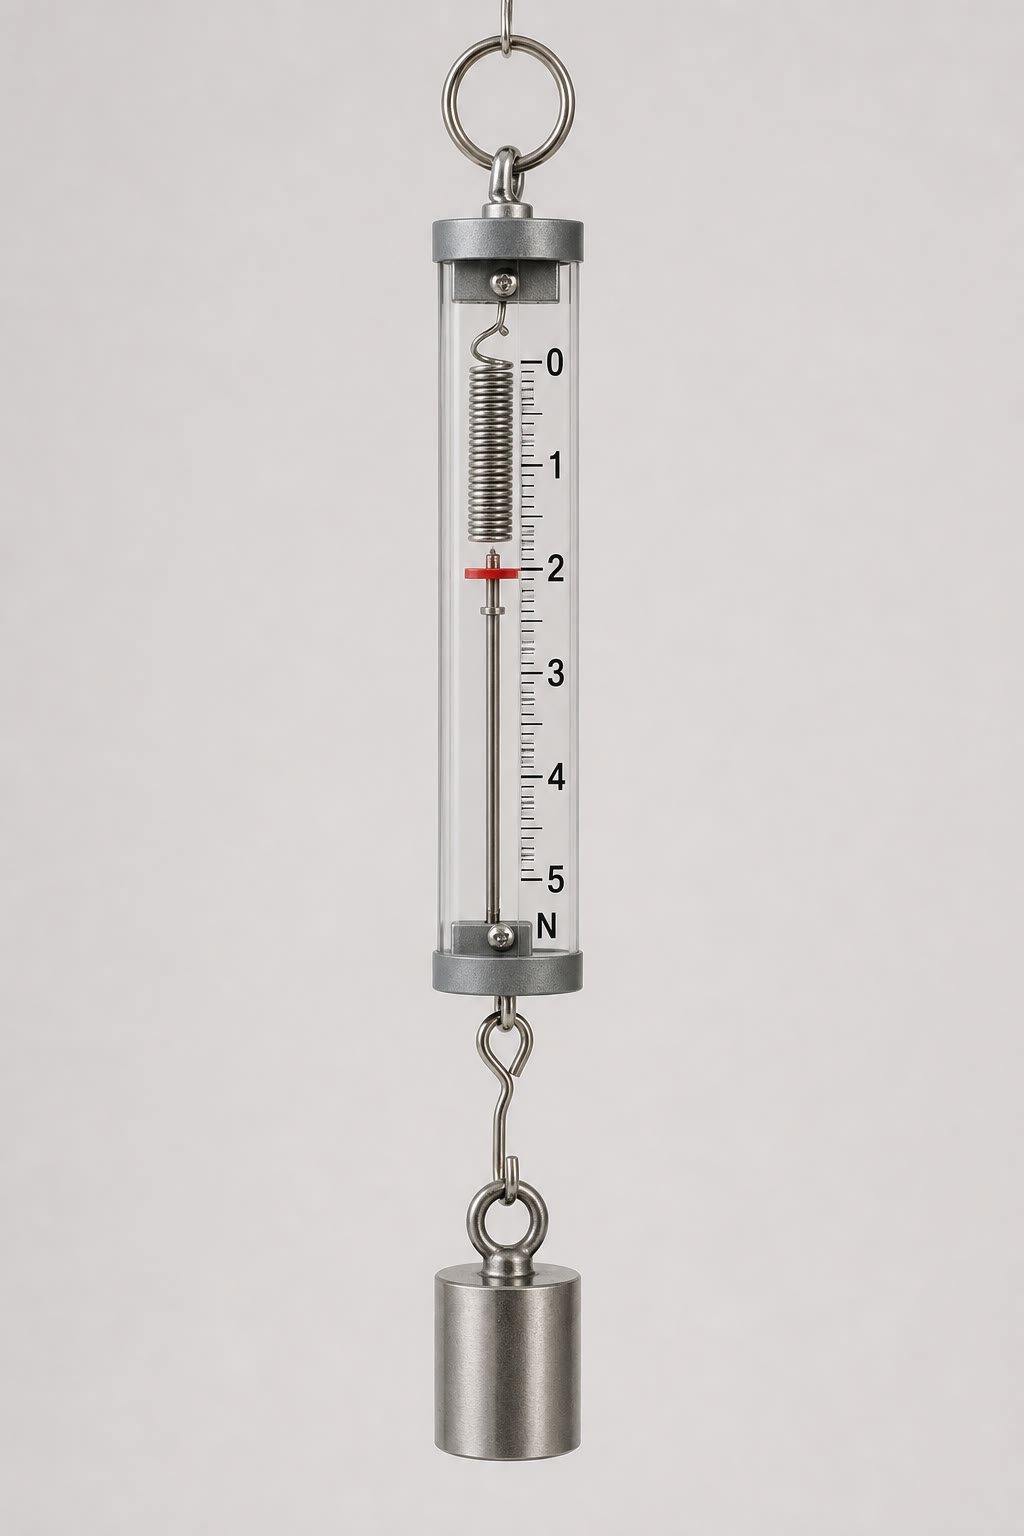
\includegraphics[width=0.3\linewidth]{images/book1/ai/g4-weight-spring-scale.jpg}

{\small \omterm{def:g4:weight-and-mass:springscale}{弹簧测力计}工作时：负载的\omterm{def:g4:weight-and-mass:weight}{重力}拉伸弹簧，指针将这一伸长转换为读数。}
\end{omfigure}

\section{月球之行}

\begin{example}[月球的拉力较弱]\label{ex:g4:weight-and-mass:moon}
\omterm{def:g2:moon-in-the-sky:moon}{月球}比地球小得多，它拉动物体的力
弱得多——大约是地球的六分之一。宇航员的背包
旅途中它的每一克\emph{\omterm{def:g3:measuring-mass:mass}{质量}}都保持不变，而它的
在\omterm{def:g2:moon-in-the-sky:moon}{月球}上的\emph{\omterm{def:g4:weight-and-mass:weight}{重力}}缩小为六分之一。这正是
蹦跳的全部秘密：原本习惯对抗地球拉力的双腿，突然要对抗
较轻的\omterm{def:g2:moon-in-the-sky:moon}{月球}拉力，于是每一步都变成了一次跳跃。
\end{example}

\begin{omfigure}
\begin{tikzpicture}[scale=0.85]
  \draw[thick] (0.2,0.9) -- (4.2,0.9);
  \draw[thick, fill=omMeth, fill opacity=0.4]
    (1.7,0.9) rectangle (2.7,1.7);
  \node[font=\footnotesize] at (2.2,1.3) {包};
  \draw[-Stealth, very thick, omDef] (2.2,0.75) -- (2.2,-0.75);
  \node[below, font=\small] at (2.2,-0.95) {地球上：拉力强};
  \draw[thick] (7.0,0.9) -- (11.0,0.9);
  \draw[thick, fill=omMeth, fill opacity=0.4]
    (8.5,0.9) rectangle (9.5,1.7);
  \node[font=\footnotesize] at (9.0,1.3) {包};
  \draw[-Stealth, very thick, omDef] (9.0,0.75) -- (9.0,0.5);
  \node[below, font=\small] at (9.0,-0.95)
    {月球上：同一个包，拉力较弱};
\end{tikzpicture}

{\small 同一个包——\omterm{def:g3:measuring-mass:mass}{质量}相同——在两个世界里。只有
拉力箭头变了：\omterm{def:g4:weight-and-mass:weight}{重力}既与所在的地方有关，
也与物体本身有关。}
\end{omfigure}

\begin{example}[月球上的两台秤]\label{ex:g4:weight-and-mass:twoscales}
把两台秤都带到\omterm{def:g2:moon-in-the-sky:moon}{月球}上，称同一个包。
\emph{弹簧}测力计如实反映所在地的情况：它的读数
小六倍——拉力确实更弱。而\emph{\omterm{def:g3:levers-and-scales:scale}{天平}}
毫无察觉：\omterm{def:g2:moon-in-the-sky:moon}{月球}拉动包，参照砝码也
\emph{同样}较弱地被拉，两盘依然平衡，它给出的
\omterm{def:g3:measuring-mass:mass}{质量}与在地球上相同。弹簧感受的是所在的地方；\omterm{def:g3:levers-and-scales:scale}{天平}比较的是
物质的多少。
\end{example}

\begin{remark}[日常用语与物理用语]\label{rem:g4:weight-and-mass:words}
在商店里，“这个瓜重一\omterm{def:g3:measuring-mass:units}{千克}”是无伤大雅的说法——
在地球上，\omterm{def:g3:measuring-mass:mass}{质量}和\omterm{def:g4:weight-and-mass:weight}{重力}总是形影不离，所以没有人会
混淆。物理学要把这两个词分开，因为它考虑的范围比
商店远得多：要研究宇航员、下落的物体，还有——在以后
的学习中——以力自身专用的\omterm{def:g2:measuring-length:measure}{单位}来度量，这个\omterm{def:g2:measuring-length:measure}{单位}
将以首先写下地球拉力定律的
科学家命名。
\end{remark}

\section{练习}

\begin{exercise}[$\star$]\label{exo:g4:weight-and-mass:1}
\omterm{def:g3:measuring-mass:mass}{质量}回答的是什么问题？\omterm{def:g4:weight-and-mass:weight}{重力}回答的是什么问题？
其中哪一个是力？
\end{exercise}

\begin{exercise}[$\star$]\label{exo:g4:weight-and-mass:2}
\omterm{def:g4:weight-and-mass:weight}{重力}总是朝哪个方向拉？哪种仪器靠
拉伸来感知\omterm{def:g4:weight-and-mass:weight}{重力}？
\end{exercise}

\begin{exercise}[$\star$]\label{exo:g4:weight-and-mass:3}
一块砖使\omterm{def:g4:weight-and-mass:springscale}{弹簧测力计}的弹簧伸长了两个手指宽。
两块相同的砖会使它伸长多少？哪一条命题
能说明这一点？
\end{exercise}

\begin{exercise}[$\star$]\label{exo:g4:weight-and-mass:4}
在
\cref{met:g4:weight-and-mass:rubberband}中的橡皮筋测力计里，
为什么要先标出空杯的位置，再往里加东西？
\end{exercise}

\begin{exercise}[$\star$]\label{exo:g4:weight-and-mass:5}
一位宇航员把一包\qty{20}{kg}的物品带到\omterm{def:g2:moon-in-the-sky:moon}{月球}上。
在那里，它的\omterm{def:g3:measuring-mass:mass}{质量}仍为\qty{20}{kg}吗？托起它
是否和在地球上一样费力？
\end{exercise}

\begin{exercise}[$\star$]\label{exo:g4:weight-and-mass:6}
为什么宇航员在\omterm{def:g2:moon-in-the-sky:moon}{月球}上能跳得这么高，
尽管背着沉重的背包？
\end{exercise}

\begin{exercise}[$\star$]\label{exo:g4:weight-and-mass:7}
在\omterm{def:g2:moon-in-the-sky:moon}{月球}上，哪一种秤的读数会改变——是\omterm{def:g4:weight-and-mass:springscale}{弹簧测力计}，还是
\omterm{def:g3:levers-and-scales:scale}{天平}？请说明每种秤实际比较或感受的是什么。
\end{exercise}

\begin{exercise}[$\star$]\label{exo:g4:weight-and-mass:8}
判断下面的说法是否正确：“一个完全没有物质的东西
在任何地方都没有\omterm{def:g4:weight-and-mass:weight}{重力}。”请用
\cref{prop:g4:weight-and-mass:morestuff}为依据，说明理由。
\end{exercise}

\begin{exercise}[$\star$]\label{exo:g4:weight-and-mass:9}
菜贩的吊秤在她往秤盘里放苹果时向\omterm{def:g1:floating-and-sinking:words}{下沉}，
她的秤感受到的是两个近亲中的哪一个？为什么她的
小伎俩在地球上仍能卖出公平的苹果\omterm{def:g3:measuring-mass:units}{千克}数？
\end{exercise}

\begin{exercise}[$\star\star$]\label{exo:g4:weight-and-mass:10}
一家太空机构必须检查探测器各部件的\omterm{def:g3:measuring-mass:mass}{质量}是否恰好
正确——但完工的探测器将在一颗遥远而较小的行星
附近工作，那里的拉力很弱。一位工程师担心：“我们在地球上的
称量结果在那里都会出错！”请安慰他：哪些
\omterm{def:g2:measuring-length:measure}{测量}结果不会随之改变，它们是用哪种仪器测出的？
\end{exercise}

\begin{exercise}[$\star\star$]\label{exo:g4:weight-and-mass:11}
在远离地球、\omterm{def:g2:moon-in-the-sky:moon}{月球}和太阳的深空中，一位宇航员
松手放开扳手：它\omterm{def:g1:floating-and-sinking:words}{漂浮}在她手边，处于失重状态。扳手
是否失去了\omterm{def:g3:measuring-mass:mass}{质量}？请给出两条日常生活中的线索，说明
她仍能察觉到物质都还在。（提示：试着摇动它，或
把它抛出去。）
\end{exercise}
